\section{Use Cases Model}
\label{sec:use_cases_model}
% Descirbes the functional requirements, mostly non-functional. During incepeion, the names of most use cases will be indentified, and perhapss 10% of teh use cases will be analyzed in detail.

\subsection{Use Cases Diagram}
\label{subsec:use_cases_diagram}
\begin{figure}[H]
%     \centering
	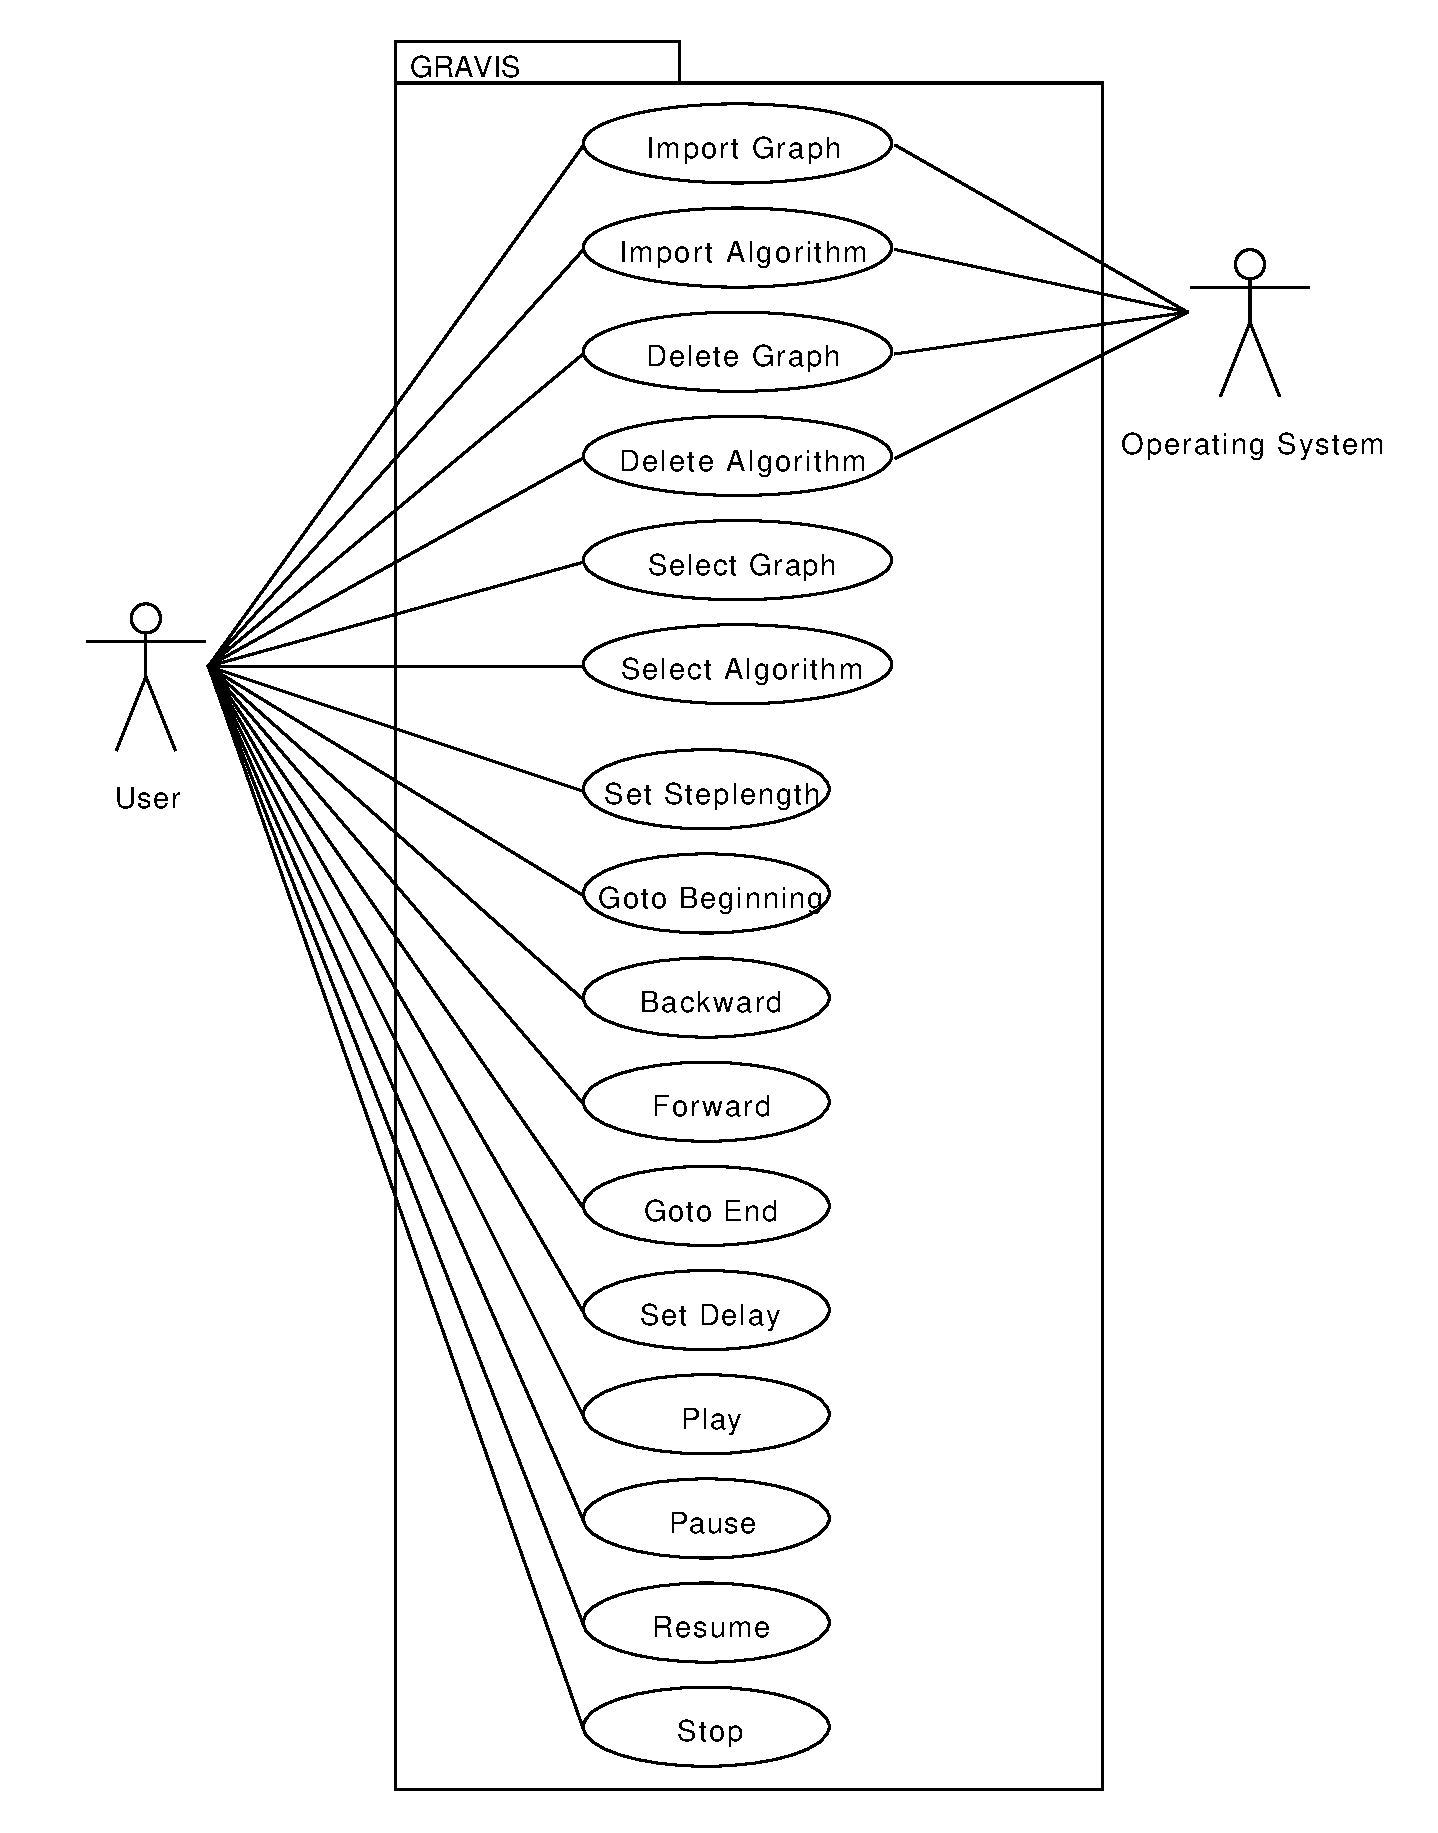
\includegraphics[scale=0.5]{diagrams/use-cases-diagram.pdf}
    \caption{Use Cases Diagram}
    \label{fig:use_cases_diagram}
\end{figure}

\subsection{Use Cases in brief format}
\label{subsec:uc_in_brief_format}
% - All the use-cases of the application you discover, which have to be written in brief format;
\begin{description}
  \item[Import Graph:] Der Benutzer kann einen neuen Graphen importieren.

  (Ausgearbeitetes Format siehe Seite~\pageref{uc:Import Graph})

  \item[Import Algorithm:] Der Benutzer kann einen neuen Algorithmus importieren.

  (Ausgearbeitetes Format siehe Seite~\pageref{uc:Import Algorithm})

  \item[Delete Graph:] Der Benutzer kann einen importierten Graphen l\"oschen.

  (Ausgearbeitetes Format siehe Seite~\pageref{uc:Delete Graph})

  \item[Delete Algorithm:] Der Benutzer kann einen importierten Algorithmus l\"oschen.

  (Ausgearbeitetes Format siehe Seite~\pageref{uc:Delete Algorithm})

  \item[Select Graph:] Der Benutzer kann einen Graphen ausw\"ahlen.

  (Ausgearbeitetes Format siehe Seite~\pageref{uc:Select Graph})

  \item[Select Algorithm:] Der Benutzer kann einen Algorithmus ausw\"ahlen, evt. Start- resp. Endknoten ausw\"ahlen.

  (Ausgearbeitetes Format siehe Seite~\pageref{uc:Select Algorithm})

  \item[Set Step:] Der Benutzer kann f\"ur die Visualisierung die Anzahl Traversierungsschritte pro Bild einstellen.

  (Ausgearbeitetes Format siehe Seite~\pageref{uc:Set Step})

  \item[Forward:] Der Benutzer kann in der Visualisierung ein Bild vorw\"arts gehen.

  (Ausgearbeitetes Format siehe Seite~\pageref{uc:Forward})

  \item[Backward:] Der Benutzer kann in der Visualisierung ein Bild r\"uckw\"arts gehen.

  (Ausgearbeitetes Format siehe Seite~\pageref{uc:Backward})

  \item[Goto Beginning:] Der Benutzer kann in der Visualisierung an das Ende springen.

  (Ausgearbeitetes Format siehe Seite~\pageref{uc:Goto Beginning})

  \item[Goto End:] Der Benutzer kann in der Visualisierung an den Anfang springen.

  (Ausgearbeitetes Format siehe Seite~\pageref{uc:Goto End})

  \item[Set Delay:] Der Benutzer kann f\"ur die Visualisierung das Zeitintervall zwischen zwei Bildern einstellen.

  (Ausgearbeitetes Format siehe Seite~\pageref{uc:Set Delay})

  \item[Play:] Der Benutzer kann das Streaming der Visualisierung starten.

  (Ausgearbeitetes Format siehe Seite~\pageref{uc:Play})

  \item[Pause:] Der Benutzer kann das Streaming der Visualisierung anhalten.

  (Ausgearbeitetes Format siehe Seite~\pageref{uc:Pause})

  \item[Resume:] Der Benutzer kann das Streaming der Visualisierung wiederaufnehmen.

  (Ausgearbeitetes Format siehe Seite~\pageref{uc:Resume})

  \item[Stop:] Der Benutzer kann das Streaming der Visualisierung stoppen.

  (Ausgearbeitetes Format siehe Seite~\pageref{uc:Stop})
\end{description}

\newpage
\subsection{Use Cases in fully dressed format}
\label{subsec:uc_in_fully_dressed_format}
F\"ur alle Use Cases gilt:
\begin{itemize}
  \item Scope: System-wide
  \item Level: User-goal
  \item Primary: Actor User
\end{itemize}
% - In addition, the use cases related to the registration and the subscription of an actor as well as the upload/download functionalities must be provided in fully-dressed format (do not forget to use the numbering as explained in the book, as well as the advices we discussed);
% 
\subsubsection{Import Graph}
\begin{usecase}{Import Graph}
    \preconditions{
	    \item Die Dateistruktur des Betriebssystems ist zug\"anglich.
	    \item Auf die zu importierende Datei sind mindestens Leserechte gesetzt.
    }
    \postconditions{
	    \item Der Graph steht dem System als Parameter zur weiteren Verarbeitung zur Verf\"ugung.
	    \item Der Graph steht dem User in der Graph-Parameterliste zur Auswahl bereit.
	    \item Der Graph wurde durch das System ausgew\"ahlt und im GUI dargestellt.
    }
    \mainsuccess{
	    \item Der Benutzer startet den \textbf{Graph-Import}.
	    \item Der Benutzer wird dazu aufgefordert, den \textbf{Pfad und den Dateinamen} einer Datei anzugeben oder den Vorgang abzubrechen.
	    \item Die angegebene Datei wird in die Dateistruktur des Systems \textbf{kopiert}.
	    \item Die angegebene Datei wird durch das System \textbf{auf Kompatibilit\"at gepr\"uft}.
	    \item Der Name des importierten Graphen wird zur Graph-\textbf{Parameterliste} hinzugef\"ugt.
	    \item Der Graph wird durch das System in der Graph-Parameterliste \textbf{ausgew\"ahlt} (siehe \textit{UC Select Graph}, Seite~\pageref{uc:Select Graph}.
    }
    \newpage
    \hline \\ [-1.3ex]
    \extensions{
	    \item[1.a]
		    \begin{enumerate}
			\item Das Starten des Vorganges \textbf{schl\"agt fehl}.
			\item Eine Fehlermeldung wird ausgegeben.
		    \end{enumerate}
	    \item[2.a]
		    \begin{enumerate}
			\item Der Benutzer \textbf{bricht den Vorgang ab}.
		    \end{enumerate}
	    \item[2.b]
		    \begin{enumerate}
			\item Die angegebene Datei kann \textbf{nicht gefunden} werden.
			\item Eine Fehlermeldung wird ausgegeben.
			\item Dem Benutzer wird widerum die M\"oglichkeit gegeben, den Pfad und den Dateinamen einer Datei anzugeben oder den Vorgang abzubrechen (Rekursion).
		    \end{enumerate}
	    \item[3.a]
		    \begin{enumerate}
			\item Die angegebene Datei \textbf{kann nicht} in die Dateistruktur des Systems \textbf{kopiert werden}.
			\item Eine Fehlermeldung wird ausgegeben.
		    \end{enumerate}
	    \item[4.a]
		    \begin{enumerate}
			\item Die angegebene Datei ist \textbf{nicht kompatibel}.
			\item Die kopierte Datei wird aus der Dateistruktur des Systems gel\"oscht.
			\item Eine Fehlermeldung wird ausgegeben.
		    \end{enumerate}
	    \item[5.a]
		    \begin{enumerate}
			\item Der Name des importierten Graphen \textbf{kann nicht zur Parameterliste hinzugef\"ugt werden}.
			\item Die kopierte Datei wird aus der Dateistruktur des Systems gel\"oscht.
			\item Eine Fehlermeldung wird ausgegeben.
		    \end{enumerate}
	    \item[6.a]
		    \begin{enumerate}
			\item siehe \textit{UC Select Graph}, Seite~\pageref{uc:Select Graph} resp. \textit{UC Select Algorithm}, Seite~\pageref{uc:Select Algorithm}.
		    \end{enumerate}
    }
\end{usecase}
\newpage 
% 
\subsubsection{Import Algorithm}
\begin{usecase}{Import Algorithm}
    \preconditions{
	    \item Die Dateistruktur des Betriebssystems ist zug\"anglich.
	    \item Auf die zu importierende Datei sind mindestens Leserechte gesetzt.
    }
    \postcondition{
	    Der Algorithmus steht dem System als Parameter zur weiteren Verarbeitung zur Verf\"ugung.
    }
    \mainsuccess{
	    \item Der Benutzer startet den \textbf{Algorithmus-Import}.
	    \item Der Benutzer wird dazu aufgefordert, den \textbf{Pfad und den Dateinamen} einer Datei anzugeben oder den Vorgang abzubrechen.
	    \item Die angegebene Datei wird in die Dateistruktur des Systems \textbf{kopiert}.
	    \item Die angegebene Datei wird durch das System \textbf{auf Kompatibilit\"at gepr\"uft}.
	    \item Der Name des importierten Parameters wird zur \textbf{Parameterliste} der entsprechenden Benutzerschnittstelle hinzugef\"ugt.
    }
    \newpage
    \hline \\ [-1.3ex]
    \extensions{
	    \item[1.a]
		    \begin{enumerate}
			\item Das Starten des Vorganges \textbf{schl\"agt fehl}.
			\item Eine Fehlermeldung wird ausgegeben.
		    \end{enumerate}
	    \item[2.a]
		    \begin{enumerate}
			\item Der Benutzer \textbf{bricht den Vorgang ab}.
		    \end{enumerate}
	    \item[2.b]
		    \begin{enumerate}
			\item Die angegebene Datei kann \textbf{nicht gefunden} werden.
			\item Eine Fehlermeldung wird ausgegeben.
			\item Dem Benutzer wird widerum die M\"oglichkeit gegeben, den Pfad und den Dateinamen einer Datei anzugeben oder den Vorgang abzubrechen (Rekursion).
		    \end{enumerate}
	    \item[3.a]
		    \begin{enumerate}
			\item Die angegebene Datei \textbf{kann nicht} in die Dateistruktur des Systems \textbf{kopiert werden}.
			\item Eine Fehlermeldung wird ausgegeben.
		    \end{enumerate}
	    \item[4.a]
		    \begin{enumerate}
			\item Die angegebene Datei ist \textbf{nicht kompatibel}.
			\item Die Datei wird aus der Dateistruktur des Systems gel\"oscht.
			\item Eine Fehlermeldung wird ausgegeben.
		    \end{enumerate}
	    \item[5.a]
		    \begin{enumerate}
			\item Der Name des importierten Parameters \textbf{kann nicht zur Parameterliste hinzugef\"ugt werden}.
			\item Der importierte Parameter wird aus dem Arbeitsspeicher gel\"oscht.
			\item Die importierte Datei wird aus der Dateistruktur des Systems gel\"oscht.
			\item Eine Fehlermeldung wird ausgegeben.
		    \end{enumerate}
	    \item[6.a]
		    \begin{enumerate}
			\item siehe \textit{UC Select Graph}, Seite~\pageref{uc:Select Graph} resp. \textit{UC Select Algorithm}, Seite~\pageref{uc:Select Algorithm}.
		    \end{enumerate}
    }
\end{usecase}
\newpage 
% 
\subsubsection{Delete Graph}
\begin{usecase}{Delete Graph}
    \precondition{
	    Der zu l\"oschende Graph steht als \textbf{Datei} zur weiteren Verarbeitung zur Verf\"ugung.
    }
    \postconditions{
	    \item Die Graph-Datei wurde aus dem System \textbf{gel\"oscht}.
	    \item Die Parameterliste wurde \textbf{aktualisiert}.
    }
    \mainsuccess{
	    \item 
    }
%     \hline \\ [-1.3ex]
    \extensions{
	    \item[1.a]
		    \begin{enumerate}
			\item 
		    \end{enumerate}
    }
\end{usecase}
\newpage 
% 
\subsubsection{Delete Algorithm}
\begin{usecase}{Delete Algorithm}
    \precondition{
	    Der zu l\"oschende Algorithmus steht als \textbf{Datei} zur weiteren Verarbeitung zur Verf\"ugung.
    }
    \postconditions{
	    \item Die Algorithmus-Datei wurde aus dem System \textbf{gel\"oscht}.
	    \item Die Parameterliste wurde \textbf{aktualisiert}.
    }
    \mainsuccess{
	    \item 
    }
%     \hline \\ [-1.3ex]
    \extensions{
	    \item[1.a]
		    \begin{enumerate}
			\item 
		    \end{enumerate}
    }
\end{usecase}
\newpage 
% 
\subsubsection{Select Graph}
\begin{usecase}{Select Graph}
    \preconditions{
	    \item Die Benutzerschnittstelle zur Wahl des Graphen ist aktiv.
    }
    \postconditions{
	    \item Der gew\"ahlte Graph steht als \textbf{geladene Instanz} zur weiteren Verarbeitung zur Verf\"ugung.
	    \item Der gew\"ahlte Graph ist visualisiert.
    }
    \mainsuccess{
	    \item In der Parameterliste wird der gew\"ahlte Graph als\textbf{aktuell} gesetzt.
	    \item Der vormalige Graph wird im System \textbf{entladen}.
	    \item Der gew\"ahlte Graph wird im System \textbf{geladen}.
	    \item Die Parameterliste zur Wahl des Algorithmus wird \textbf{angepasst}.
	    \item Als Visualisierung wird der aktuelle Graph gezeichnet.
    }
%     \hline \\ [-1.3ex]
    \extensions{
	    \item[1.a]
		    \begin{enumerate}
			\item Das Setzen des gew\"ahlten Graphen als aktuell \textbf{schl\"agt fehl}.
			\item Eine Fehlermeldung wird ausgegeben.
		    \end{enumerate}
	    \item[2.a]
		    \begin{enumerate}
			\item Der vormalige Graph kann \textbf{nicht entladen} werden.
			\item In der Parameterliste wird der vormalige Graph als aktuell gesetzt.
			\item Eine Fehlermeldung wird ausgegeben.
		    \end{enumerate}
	    \item[3.a]
		    \begin{enumerate}
			\item Der gew\"ahlte Graph kann \textbf{nicht geladen} werden.
			\item In der Parameterliste Graph wird ein leerer Default-Wert als aktuell gesetzt.
			\item Eine Fehlermeldung wird ausgegeben.
		    \end{enumerate}
    }
\end{usecase}
\newpage 
% 
\subsubsection{Select Algorithm}
\begin{usecase}{Select Algorithm}
    \preconditions{
	    \item Die Benutzerschnittstelle zur Wahl des Algorithmus ist aktiv.
    }
    \postconditions{
	    \item Der gew\"ahlte Algorithmus steht als \textbf{geladene Instanz} zur weiteren Verarbeitung zur Verf\"ugung.
    }
    \mainsuccess{
	    \item In der Parameterliste wird der gew\"ahlte Algorithmus als \textbf{aktuell} gesetzt.
	    \item Der vormalige Algorithmus wird im System \textbf{entladen}.
	    \item Der gew\"ahlte Algorithmus wird im System \textbf{geladen}.
    }
%     \hline \\ [-1.3ex]
    \extensions{
	    \item[1.a]
		    \begin{enumerate}
			\item Das Setzen des gew\"ahlten Algorithmus als aktuell \textbf{schl\"agt fehl}.
			\item Eine Fehlermeldung wird ausgegeben.
		    \end{enumerate}
	    \item[2.a]
		    \begin{enumerate}
			\item Der vormalige Algorithmus kann \textbf{nicht entladen} werden.
			\item In der Parameterliste wird der vormalige Algorithmus als aktuell gesetzt.
			\item Eine Fehlermeldung wird ausgegeben.
		    \end{enumerate}
	    \item[3.a]
		    \begin{enumerate}
			\item Der gew\"ahlte Algorithmus kann \textbf{nicht geladen} werden.
			\item In der Parameterliste wird ein leerer Default-Wert als aktuell gesetzt.
			\item Eine Fehlermeldung wird ausgegeben.
		    \end{enumerate}
    }
\end{usecase}
\newpage 
% 
\subsubsection{Set Step}
\begin{usecase}{Set Step}
    \precondition{
	    
    }
    \postconditions{
	    \item 
	    \item 
    }
    \mainsuccess{
	    \item 
    }
%     \hline \\ [-1.3ex]
    \extensions{
	    \item[1.a]
		    \begin{enumerate}
			\item 
		    \end{enumerate}
    }
\end{usecase}
\newpage 
% 
\subsubsection{Forward}
\begin{usecase}{Forward}
    \precondition{
	    
    }
    \postconditions{
	    \item 
	    \item 
    }
    \mainsuccess{
	    \item 
    }
%     \hline \\ [-1.3ex]
    \extensions{
	    \item[1.a]
		    \begin{enumerate}
			\item 
		    \end{enumerate}
    }
\end{usecase}
\newpage 
% 
\subsubsection{Backward}
\begin{usecase}{Backward}
    \precondition{
	    
    }
    \postconditions{
	    \item 
	    \item 
    }
    \mainsuccess{
	    \item 
    }
%     \hline \\ [-1.3ex]
    \extensions{
	    \item[1.a]
		    \begin{enumerate}
			\item 
		    \end{enumerate}
    }
\end{usecase}
\newpage 
% 
\subsubsection{Goto Beginning}
\begin{usecase}{Goto Beginning}
    \precondition{
	    
    }
    \postconditions{
	    \item 
	    \item 
    }
    \mainsuccess{
	    \item 
    }
%     \hline \\ [-1.3ex]
    \extensions{
	    \item[1.a]
		    \begin{enumerate}
			\item 
		    \end{enumerate}
    }
\end{usecase}
\newpage 
% 
\subsubsection{Goto End}
\begin{usecase}{Goto End} 

    \precondition{
	    
    }
    \postconditions{
	    \item 
	    \item 
    }
    \mainsuccess{
	    \item 
    }
%     \hline \\ [-1.3ex]
    \extensions{
	    \item[1.a]
		    \begin{enumerate}
			\item 
		    \end{enumerate}
    }
\end{usecase}
\newpage 
% 
\subsubsection{Set Delay}
\begin{usecase}{Set Delay}
    \precondition{
	    
    }
    \postconditions{
	    \item 
	    \item 
    }
    \mainsuccess{
	    \item 
    }
%     \hline \\ [-1.3ex]
    \extensions{
	    \item[1.a]
		    \begin{enumerate}
			\item 
		    \end{enumerate}
    }
\end{usecase}
\newpage 
% 
\subsubsection{Play}
\begin{usecase}{Play}
    \precondition{
	    
    }
    \postconditions{
	    \item 
	    \item 
    }
    \mainsuccess{
	    \item 
    }
%     \hline \\ [-1.3ex]
    \extensions{
	    \item[1.a]
		    \begin{enumerate}
			\item 
		    \end{enumerate}
    }
\end{usecase}
\newpage 
% 
\subsubsection{Pause}
\begin{usecase}{Pause}
    \precondition{
	    
    }
    \postconditions{
	    \item 
	    \item 
    }
    \mainsuccess{
	    \item 
    }
%     \hline \\ [-1.3ex]
    \extensions{
	    \item[1.a]
		    \begin{enumerate}
			\item 
		    \end{enumerate}
    }
\end{usecase}
\newpage 
% 
\subsubsection{Resume}
\begin{usecase}{Resume}
    \precondition{
	    
    }
    \postconditions{
	    \item 
	    \item 
    }
    \mainsuccess{
	    \item 
    }
%     \hline \\ [-1.3ex]
    \extensions{
	    \item[1.a]
		    \begin{enumerate}
			\item 
		    \end{enumerate}
    }
\end{usecase}
\newpage 
% 
\subsubsection{Stop}
\begin{usecase}{Stop}
    \precondition{
	    
    }
    \postconditions{
	    \item 
	    \item 
    }
    \mainsuccess{
	    \item 
    }
%     \hline \\ [-1.3ex]
    \extensions{
	    \item[1.a]
		    \begin{enumerate}
			\item 
		    \end{enumerate}
    }
\end{usecase}
\newpage
% 

Der Visualisierungsfortschritt wird in der Progressbar angezeigt.